\chapter{样式与组件总览(Sampler)}

本章汇集了常用的版式元素,便于快速检查“教材风”样式在你的环境下的呈现效果:标题、段落、列表、代码高亮、盒子、表格、长表格与 TikZ 简图等。

\section{标题层级与段落}
这是一个普通段落。中文采用宋体(Noto Serif CJK SC),英文采用 Libertinus Serif。默认首行缩进两字符,段间距为 0,行距 1.25。Inline code 示例:\texttt{mov ds, ax}、\texttt{0x7C00}。

\subsection{小节标题}
小节风格紧凑,不占过多垂直空间。再来一个段落,用于观察换行与对齐效果。

\subsubsection{小小节标题}
说明性文本,继续观察标题与正文之间的间距与对比度是否符合“教材感”。

\section{列表}
\begin{itemize}
  \item 无序列表项 A
  \item 无序列表项 B
\end{itemize}

\begin{enumerate}
  \item 有序列表项 1
  \item 有序列表项 2
\end{enumerate}

\section{提示/警告盒子}
\begin{notebox}[title=注意]
使用 \verb|\notebox| 呈现普通提示;白底、浅灰边。可放入简短定义或引导性说明。
\end{notebox}

\begin{warnbox}[title=警告]
用于重要风险提示,例如“写盘会覆盖镜像”。
\end{warnbox}

\begin{tipbox}[title=提示]
用于辅助信息或技巧,比如“Bochs 日志可用 \verb|\codefile| 引入片段用于记录实验证据”。
\end{tipbox}

\section{代码高亮(minted)}
\subsection{C++ 片段}
\begin{codeblock}[示例:C++]{c++}
#include <cstdint>
auto sum(int a, int b) -> int {
    return a + b;
}
\end{codeblock}

\subsection{NASM 片段}
\begin{codeblock}[示例:NASM]{nasm}
BITS 16
org 0x7C00
cli
xor ax, ax
mov ds, ax
sti
\end{codeblock}

\subsection{引用仓库文件(前 40 行)}
\codefile[firstline=1,lastline=40]{nasm}{../kernel/interrupt.asm}

\section{表格与长表格}
\subsection{普通表格}
\begin{table}[h]
  \centering
  \begin{tabular}{ll}
    \toprule
    符号 & 说明 \\
    \midrule
    GDT & 全局描述符表 \\
    IDT & 中断描述符表 \\
    TSS & 任务状态段 \\
    \bottomrule
  \end{tabular}
  \caption{核心数据结构缩略语}
\end{table}

\subsection{长表格(示例)}
\begin{longtable}{lll}
  \caption{中断向量片段(示意)}\\
  \toprule 向量 & 类型 & 说明 \\
  \midrule
  \endfirsthead
  \toprule 向量 & 类型 & 说明 \\
  \midrule
  \endhead
  0x00 & 异常 & 除零错误 \\
  0x01 & 异常 & 调试 \\
  0x20 & 外设 & PIT 定时器 \\
  0x21 & 外设 & 键盘 \\
  0x80 & 系统调用 & 用户态陷入 \\
  \bottomrule
\end{longtable}

\section{TikZ 简图:内存布局(示意)}
\begin{center}
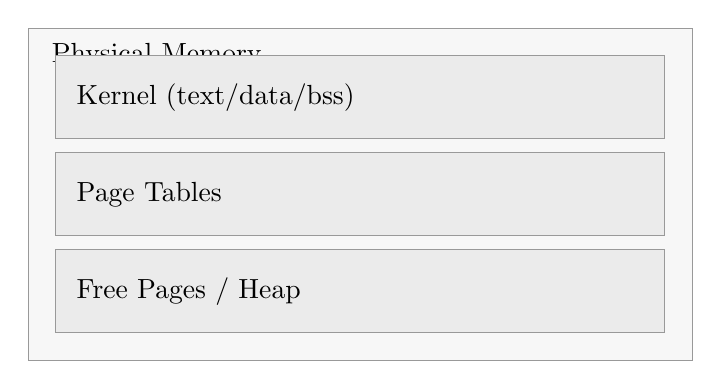
\begin{tikzpicture}[x=1pt,y=1pt]
  \draw[fill=black!3,draw=black!40] (0,0) rectangle (240,120);
  \node[anchor=west] at (5,110) {Physical Memory};
  % Regions
  \draw[fill=black!8,draw=black!40] (10,80) rectangle (230,110);
  \node[anchor=west] at (14,95) {Kernel (text/data/bss)};
  \draw[fill=black!8,draw=black!40] (10,45) rectangle (230,75);
  \node[anchor=west] at (14,60) {Page Tables};
  \draw[fill=black!8,draw=black!40] (10,10) rectangle (230,40);
  \node[anchor=west] at (14,25) {Free Pages / Heap};
\end{tikzpicture}
\end{center}
